\let\negmedspace\undefined
\let\negthickspace\undefined
\documentclass[journal,12pt,onecolumn]{IEEEtran}
\usepackage{cite}
\usepackage{amsmath,amssymb,amsfonts,amsthm}
\usepackage{amsmath}
\usepackage{algorithmic}
\usepackage{graphicx}
\usepackage{textcomp}
\usepackage{xcolor}
\usepackage{txfonts}
\usepackage{listings}
\usepackage{multicol}
\usepackage{enumitem}
\usepackage{mathtools}
\usepackage{gensymb}
\usepackage{comment}
\usepackage[breaklinks=true]{hyperref}
\usepackage{tkz-euclide} 
\usepackage{listings}
\usepackage{gvv}                                        
\usepackage[latin1]{inputenc}                                
\usepackage{color}                                            
\usepackage{array}                                            
\usepackage{longtable}                                       
\usepackage{calc}                                             
\usepackage{multirow}                                         
\usepackage{hhline}                                           
\usepackage{ifthen}                                           
\usepackage{lscape}
\usepackage{tabularx}
\usepackage{array}
\usepackage{float}
\usepackage{tikz}
\usepackage{multicol}
\usepackage{circuitikz}
\usetikzlibrary{patterns}
\newtheorem{theorem}{Theorem}[section]
\newtheorem{problem}{Problem}
\newtheorem{proposition}{Proposition}[section]
\newtheorem{lemma}{Lemma}[section]
\newtheorem{corollary}[theorem]{Corollary}
\newtheorem{example}{Example}[section]
\newtheorem{definition}[problem]{Definition}
\newcommand{\BEQA}{\begin{eqnarray}}
\newcommand{\EEQA}{\end{eqnarray}}
\newcommand{\define}{\stackrel{\triangle}{=}}
\theoremstyle{remark}
\newtheorem{rem}{Remark}

\begin{document}

\bibliographystyle{IEEEtran}
\vspace{3cm}

\title{2023-XE}
\author{EE24BTECH11020 -  Ellanti Rohith}
\maketitle

\renewcommand{\thefigure}{\theenumi}
\renewcommand{\thetable}{\theenumi}
\section*{General Aptitude (GA)}




\begin{enumerate}
    \item The second smallest eigenvalue of the eigenvalue problem
    \begin{align*}
    \dfrac{d^2 y}{dx^2} + (\lambda - 3)y = 0, \quad y(0) = y(\pi) = 0,
    \end{align*}
    is\hfill{[GATE 2023]}
    \begin{multicols}{4}
    \begin{enumerate}
        \item $4$
        \item $3$
        \item $7$
        \item $9$
    \end{enumerate}
    \end{multicols}

    \item Which one of the following functions is differentiable at $z = 0$ but \textbf{NOT} differentiable at any other point in the complex plane $\mathbb{C}$?\hfill{[GATE 2023]}
    \begin{multicols}{2}
    \begin{enumerate}
        \item $f\brak{z} = z |z|, \quad z \in \mathbb{C}$
        
        \item $f\brak{z} = \begin{cases} \frac{1}{e^z}, & z \neq 0 \\ 0, & z = 0 \end{cases}, \quad z \in \mathbb{C}$\item $f\brak{z} = \sin\brak{z}, \quad z \in \mathbb{C}$
        \item $f\brak{z} = e^{-z^2}, \quad z \in \mathbb{C}$
    \end{enumerate}
    \end{multicols}

    \item If the polynomial
    \begin{align*}
    P(x) = a_0 + a_1 x + a_2 x (x - 1) + a_3 x (x - 1)(x - 2)
    \end{align*}
    interpolates the points $(0,2)$, $(1,3)$, $(2,2)$, and $(3,5)$, then the value of $P\left(\dfrac{5}{2}\right)$ is \underline{\hspace{1cm}} (round off to 2 decimal places).\hfill{[GATE 2023]}

    \item The value of $m$ for which the vector field
    \begin{align*}
    \vec{F}(x, y) = (4x^m y^2 - 2 x y^m) \hat{i} + (2x^4 y - 3x^2 y^2) \hat{j}
    \end{align*}
  is a conservative vector field, is \underline{\hspace{1cm}} (in integer).\hfill{[GATE 2023]}
\item Let
    \begin{align*}
    P = \myvec{ 4 & -2 & 2 \\ 6 & -3 & 4 \\ 3 & -2 & 3 } \quad \text{and} \quad Q = \myvec{ 3 & -2 & 2 \\ 4 & -4 & 6 \\ 2 & -3 & 5 }.
    \end{align*}
    The eigenvalues of both $P$ and $Q$ are $1$, $1$, and $2$. Which one of the following statements is TRUE?\hfill{[GATE 2023]}
   
    \begin{enumerate}
        \item Both $P$ and $Q$ are diagonalizable
        \item $P$ is diagonalizable but $Q$ is NOT diagonalizable
        \item $P$ is NOT diagonalizable but $Q$ is diagonalizable
        \item Both $P$ and $Q$ are NOT diagonalizable
    \end{enumerate}
   

    \item The surface area of the portion of the paraboloid
    \begin{align*}
    z = x^2 + y^2
    \end{align*}
    that lies between the planes $z = 0$ and $z = \dfrac{1}{4}$ is\hfill{[GATE 2023]}
    \begin{multicols}{4}
    \begin{enumerate}
        \item $\dfrac{\pi}{6} (2\sqrt{2} - 1)$
        \item $\dfrac{\pi}{2} (2\sqrt{2} - 1)$
        \item $\pi (2\sqrt{2} - 1)$
        \item $\dfrac{\pi}{3} (2\sqrt{2} - 1)$
    \end{enumerate}
    \end{multicols}

    \item The probability of a person telling the truth is $\dfrac{4}{6}$. An unbiased die is thrown by the same person twice and the person reports that the numbers appeared in both the throws are the same. Then the probability that actually the numbers appeared in both the throws are same is \underline{\hspace{1cm}} (round off to 2 decimal places).\hfill{[GATE 2023]}

    \item Let $u(x, t)$ be the solution of the initial boundary value problem
    \begin{align*}
    \dfrac{\partial u}{\partial t} = \dfrac{\partial^2 u}{\partial x^2}, \quad x \in (0, 2), \, t > 0
    \end{align*}
    \begin{align*}
    u(x, 0) = \sin(\pi x), \quad x \in (0, 2)
    \end{align*}
    \begin{align*}
    u(0, t) = u(2, t) = 0.
    \end{align*}
    Then the value of $e^{\pi^2} \left( u\left( \dfrac{1}{2}, 1 \right) - u\left( \dfrac{3}{2}, 1 \right) \right)$ is \underline{\hspace{1cm}} (in integer).\hfill{[GATE 2023]}
     \item Match the following measuring instruments with the appropriate figures.\hfill{[GATE 2023]}
    \begin{enumerate}
    \item[I.] Pitot probe
        \item[II.] Pitot-static probe
        \item[III.] Piezometer
    \end{enumerate}
    


    \begin{multicols}{2}
    \begin{enumerate}
        \item I -- P; II -- Q; III -- R
        \item I -- R; II -- Q; III -- P
        \item I -- R; II -- P; III -- Q
        \item I -- Q; II -- P; III -- R
    \end{enumerate}
    \end{multicols}

    \item Among the following non-dimensional numbers, which one characterizes periodicity present in a transient flow?\hfill{[GATE 2023]}
    
    
     \begin{multicols}{2}
    \begin{enumerate}
 \item 
\begin{tikzpicture}
            \fill[gray] (0,0) -- (-0.5,1) -- (1,1) -- (1.5,0)-- cycle;
              \fill[gray] (0,0) -- (-0.5,-1) -- (1,-1) -- (1.5,0) -- cycle;
        \end{tikzpicture}        
        \item 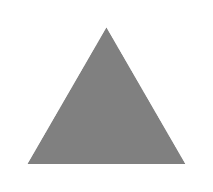
\begin{tikzpicture}
            \fill[gray] (0,0) -- (1,1.73) -- (2,0) -- cycle;
        \end{tikzpicture}
       \item 
\begin{tikzpicture}
            \fill[gray] (0,0) -- (2.2,0) -- (1.85,1.5) -- (0.35,1.5) -- cycle; 
            
        \end{tikzpicture}
        \item  
\begin{tikzpicture}
            \fill[gray] (0,0) rectangle (2,2);
        \end{tikzpicture}
        
        
    \end{enumerate}
    \end{multicols}
    
 \hspace{5cm}(P)\hspace{5cm}(Q)\hspace{5cm} (R)
    \begin{multicols}{2}
    \begin{enumerate}
        \item Froude number
        \item Strouhal number
        \item Peclet number
        \item Lewis number
    \end{enumerate}
    \end{multicols}

    \item For an incompressible boundary layer flow over a flat plate shown in the figure, the momentum thickness is expressed as
  \begin{center}
\resizebox{0.6\textwidth}{!}{%
\begin{circuitikz}
\tikzstyle{every node}=[font=\large]
\draw (2.5,13) to[short] (2.5,6);
\draw (2.5,6) to[short] (11.25,6);
\draw (11.25,13) to[short] (11.25,6);
\draw [color={rgb,255:red,0; green,128; blue,0}](2.5,6.5) to[short] (11.25,6.5);
\draw [ color={rgb,255:red,255; green,0; blue,0}, dashed] (3,12.75) .. controls (3,9.25) and (5.5,7) .. (11.25,10.5);
\draw [color={rgb,255:red,0; green,0; blue,255}, dashed] (3,12.75) .. controls (3.5,6) and (5.25,7.75) .. (11.5,7);
\draw [ color={rgb,255:red,128; green,0; blue,128}, dashdotted] (2.5,6) -- (11.25,9.75);
\node [font=\large, rotate around={90:(0,0)}] at (2.1,9.5) {$Cost\text{ } per\text{ } unit \rightarrow$};
\node [font=\large] at (7.75,5.5) {$Order\text{ } quantity \rightarrow$};
\node [font=\normalsize, color={rgb,255:red,255; green,0; blue,0}] at (9.25,10.75) {$Curve \, P1$};
\node [font=\normalsize, color={rgb,255:red,128; green,0; blue,128}] at (10.5,8.5) {$Curve \, P2$};
\node [font=\normalsize, color={rgb,255:red,0; green,0; blue,255}] at (8.75,8) {$Curve \, P3$};
\node [font=\normalsize, color={rgb,255:red,0; green,128; blue,0}] at (5.75,7) {$Curve \, P4$};
\draw [->, >=Stealth] (6.5,7) -- (7.75,6.5);
\draw [->, >=Stealth] (9,7.75) -- (9.5,7.25);
\draw [->, >=Stealth] (9.25,10.5) -- (9.5,9.75);
\draw [->, >=Stealth] (10.5,8.75) -- (10,9.25);
\end{circuitikz}
}%
\end{center}\hfill{[GATE 2023]}
    \begin{multicols}{2}
    \begin{enumerate}
        \item $\int_0^{\infty} \dfrac{u}{U_\infty} \, dy$
        \item $\int_0^{\infty} \left( 1 - \dfrac{u}{U_\infty} \right) dy$
        \item $\int_0^{\infty} \dfrac{u}{U_\infty} \left( 1 - \dfrac{u}{U_\infty} \right) dy$
        \item $\int_0^{\infty} \left( 1 - \dfrac{u^2}{U_\infty^2} \right) dy$
    \end{enumerate}
    \end{multicols}
    \section*{(Fluid Mechanics)}
    \item Among the shear stress versus shear strain rate curves shown in the figure, which one corresponds to a shear thinning fluid?



\resizebox{0.2\textwidth}{!}{%
\begin{circuitikz}
\tikzstyle{every node}=[font=\LARGE]
\draw  (6.25,10.5) circle (1.75cm);
\draw  (6.25,10.5) circle (0.5cm);
\draw  (6,11.75) rectangle (6.5,11.5);
\draw  (7.5,10.75) rectangle (7.75,10);
\draw  (6,9.5) rectangle (6.5,9.25);
\draw  (4.75,10.75) rectangle (5,10);
\end{circuitikz}
}%
\hfill{[GATE 2023]}
\begin{enumerate}
    \item $P$
    \item $Q$
    \item $R$
    \item $S$
\end{enumerate}


\item Consider steady incompressible flow over a flat plate, where the dashed line represents the edge of the boundary layer, as shown in the figure. Which one among the following statements is true?\hfill{[GATE 2023]}

\begin{center}
\begin{figure}[!ht]
\centering
\resizebox{0.27\textwidth}{!}{%
\begin{circuitikz}
\tikzstyle{every node}=[font=\normalsize]
\draw [->, >=Stealth] (1.25,9.25) -- (5,9.25);
\draw [->, >=Stealth] (1.25,9.25) -- (1.25,13.25);
\node [font=\normalsize, rotate around={90:(0,0)}] at (0.75,11.25) {Stress};
\node [font=\normalsize] at (3.25,9) {Strain};
\draw [->, >=Stealth] (1.25,9.25) -- (2.5,10.5);
\draw [->, >=Stealth] (4.5,12.5) -- (3.25,11.25);
\draw (2.5,10.5) to[short] (3.25,11.25);
\end{circuitikz}
}%

\end{figure}

\end{center}

\begin{enumerate}
    \item Bernoulli's equation can be applied in Region I between any two arbitrary points.
    \item Bernoulli's equation can be applied in Region I only along a streamline.
    \item Bernoulli's equation cannot be applied in Region II.
    \item Bernoulli's equation cannot be applied in Region I.
\end{enumerate}
\end{enumerate}

\end{document}